\section{Modeling and Specification}

Formal modeling use notations and tools from mathematics to be precise. Formal models enable the use of automatic analysis. They are good at finding ill-formed examples and checking properties. \\

Alloy is a formal modeling language based on set theory. An alloy model specifies a collection of constraints. The alloy analyzer takes the constraints of a model and tries to find a structure that satisfies them. There are three levels of abstraction in alloy: the object oriented paradigm, set theory, and atoms and relations.\\

There are four key ideas:
\begin{itemize}
	\item Everything is a relation. All data types and structures are relations. A key operator is dot join.
	\item Non-specialized logic. No special constructs for state machines, traces, synchronization, concurrency etc.
	\item Counterexamples \& Scope. Observations about design analysis: most assertions are wrong and most flaws have small counterexamples.
	\item Analysis by SAT. SAT is easy, so reduce the problem to SAT.
\end{itemize}


\subsection{Logic}

Atoms are alloy's primitive entities (indivisible, immutable and uninterpreted). Relations are use to associate atoms with one another. Every value in alloy logic is a relation.\\

Sets are unary relations, scalars are singleton sets and binary relations are sets of two columns. For these relations it holds that rows are unordered while columns are ordered but unnamed. Further, all relations are first order relations, meaning they cannot contains other relations (no set of sets).\\

We have the following constants: \texttt{none} is the empty set, \texttt{univ} is the universal set and \texttt{iden} is the identity relation.

\subsubsection{Operators}

\textbf{Set Operators}
\begin{center}
	\begin{tabular}{l l}
  		\texttt{+} & union \\
  		\texttt{\&} & intersection \\
  		\texttt{-} & difference \\
  		\texttt{in} & subset \\
  		\texttt{=} & equality \\
  		\texttt{->} & cross product
	\end{tabular}
\end{center}

\textbf{Join Operators}

\texttt{.}  dot join, column that is joind on is left out of the result\\
\texttt{[]} box join, \texttt{a.b.c[d] = d.(a.b.c)}\\

\textbf{Restriction and Override}
\begin{center}
	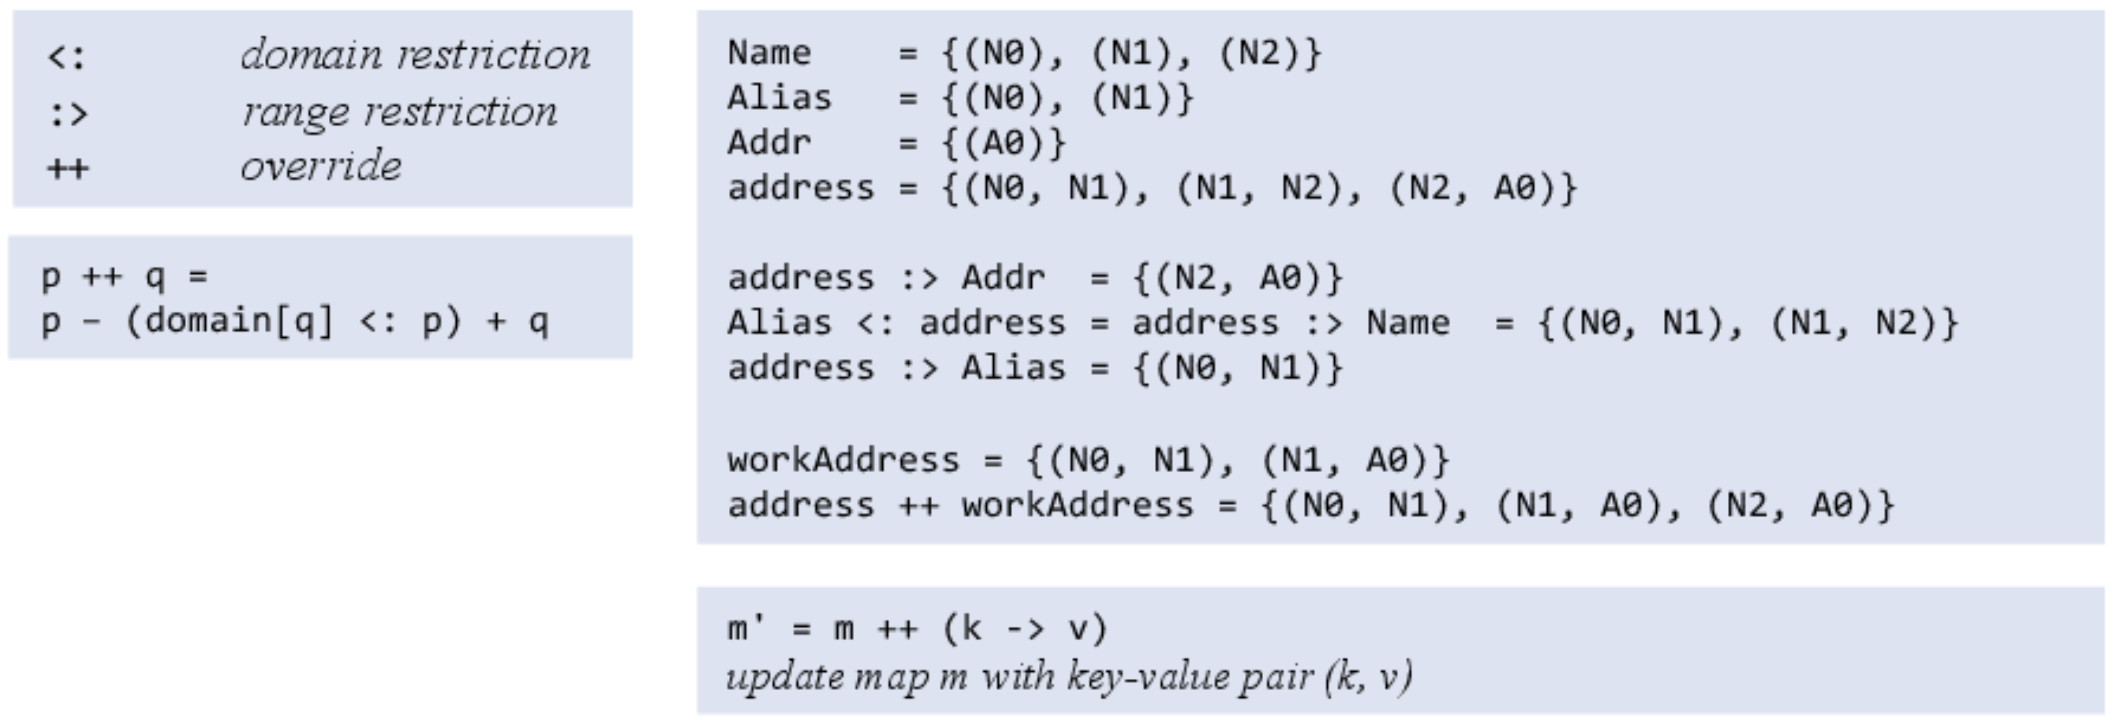
\includegraphics[width=\columnwidth]{assets/restriction}
\end{center}

\vspace{-8pt}
\textbf{Unary Operators}
\begin{center}
	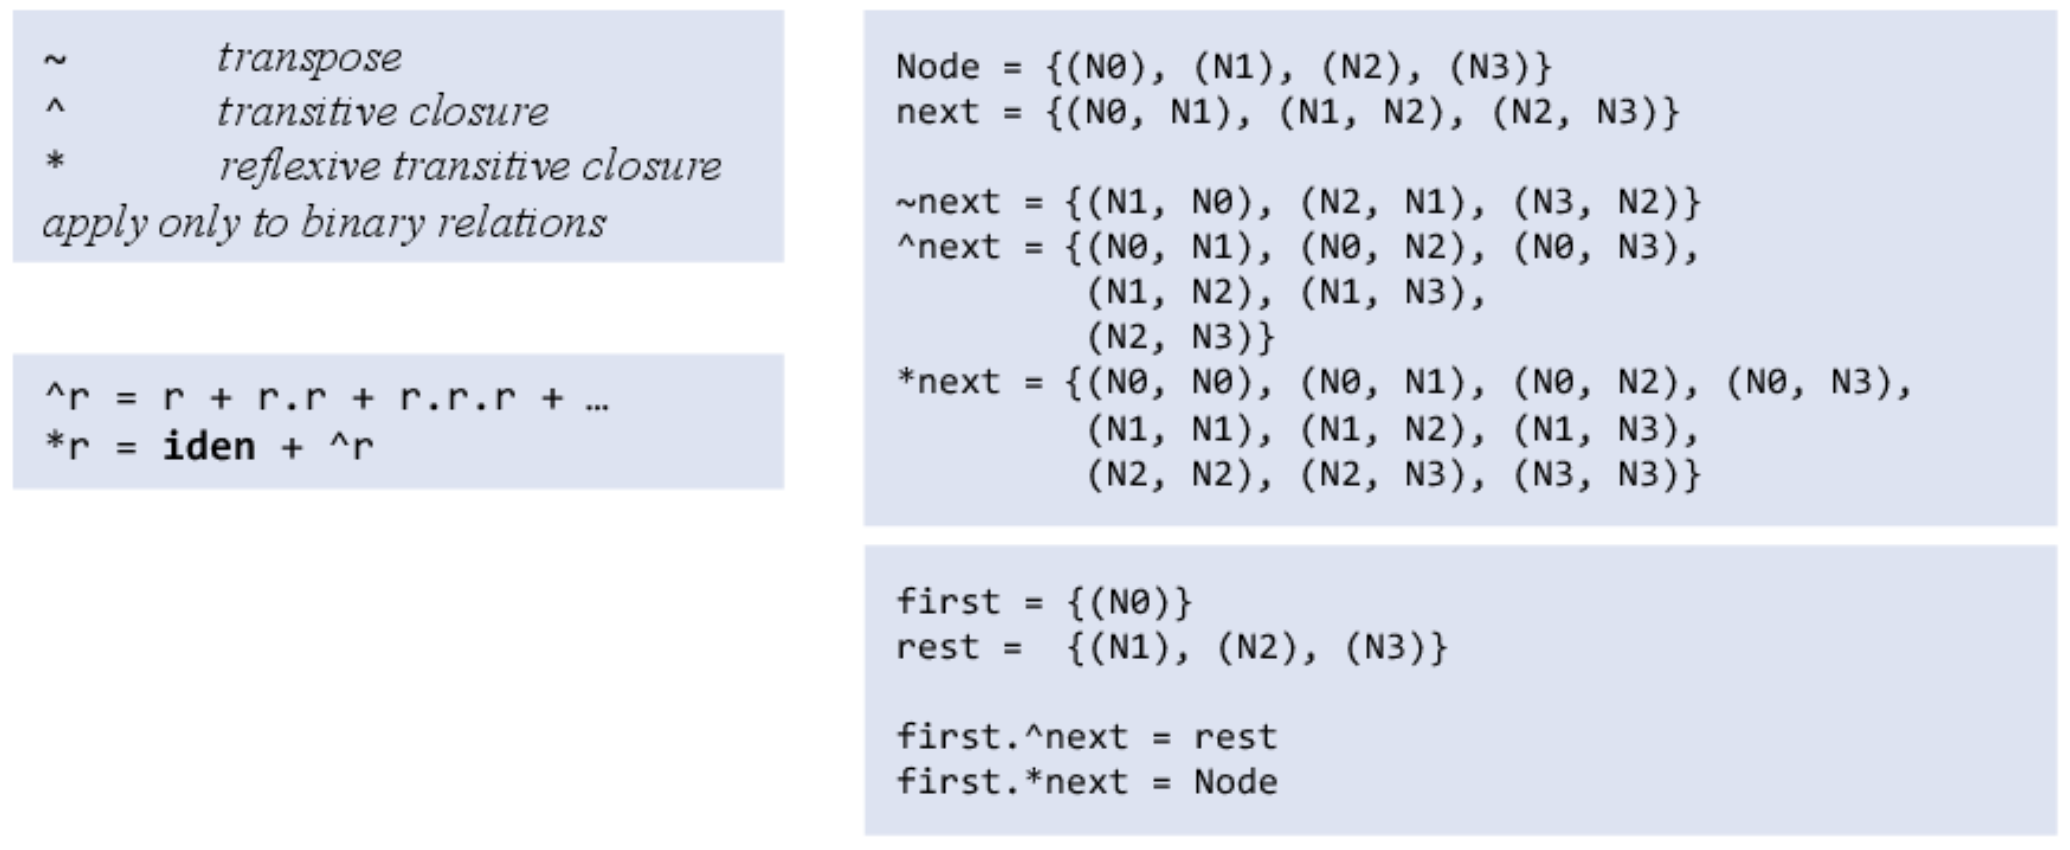
\includegraphics[width=\columnwidth]{assets/unary}
\end{center}

\vspace{-8pt}
\textbf{Boolean Operators}
\begin{center}
	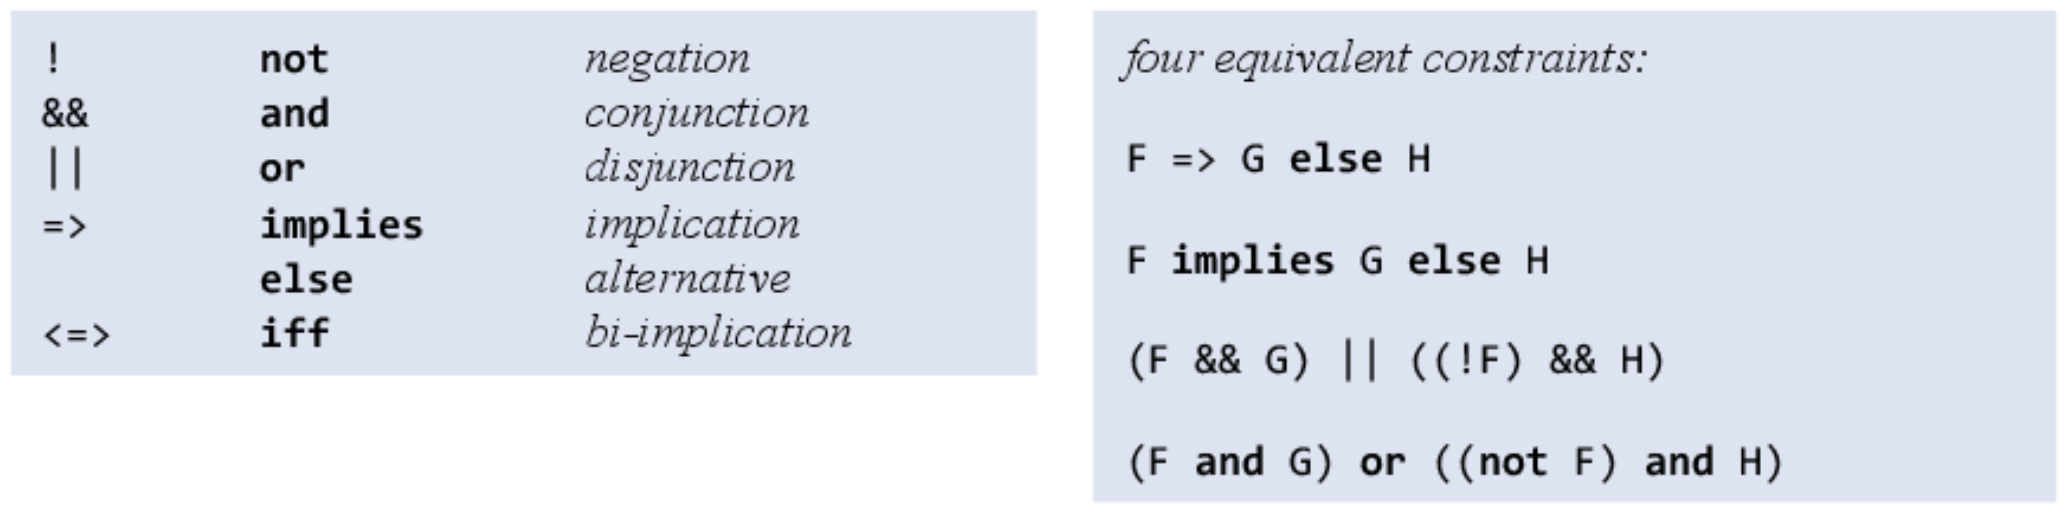
\includegraphics[width=\columnwidth]{assets/boolean}
\end{center}

\vspace{-8pt}
\textbf{Quantifiers}
\begin{center}
	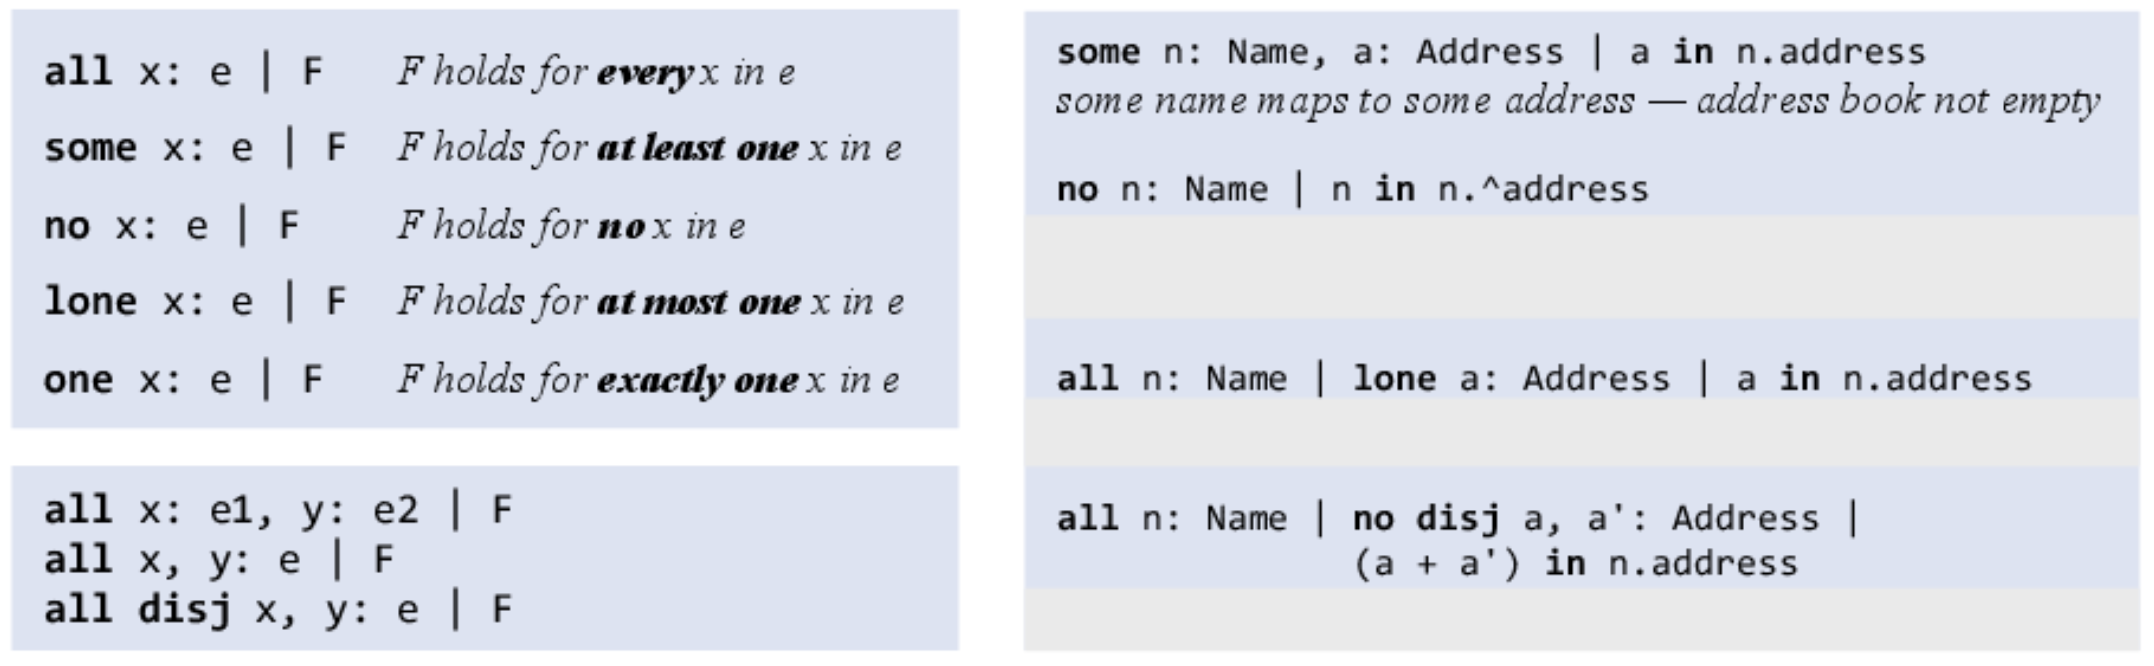
\includegraphics[width=\columnwidth]{assets/quantifiers}
\end{center}

\vspace{-4pt}
\textbf{If and Let}
\begin{center}
	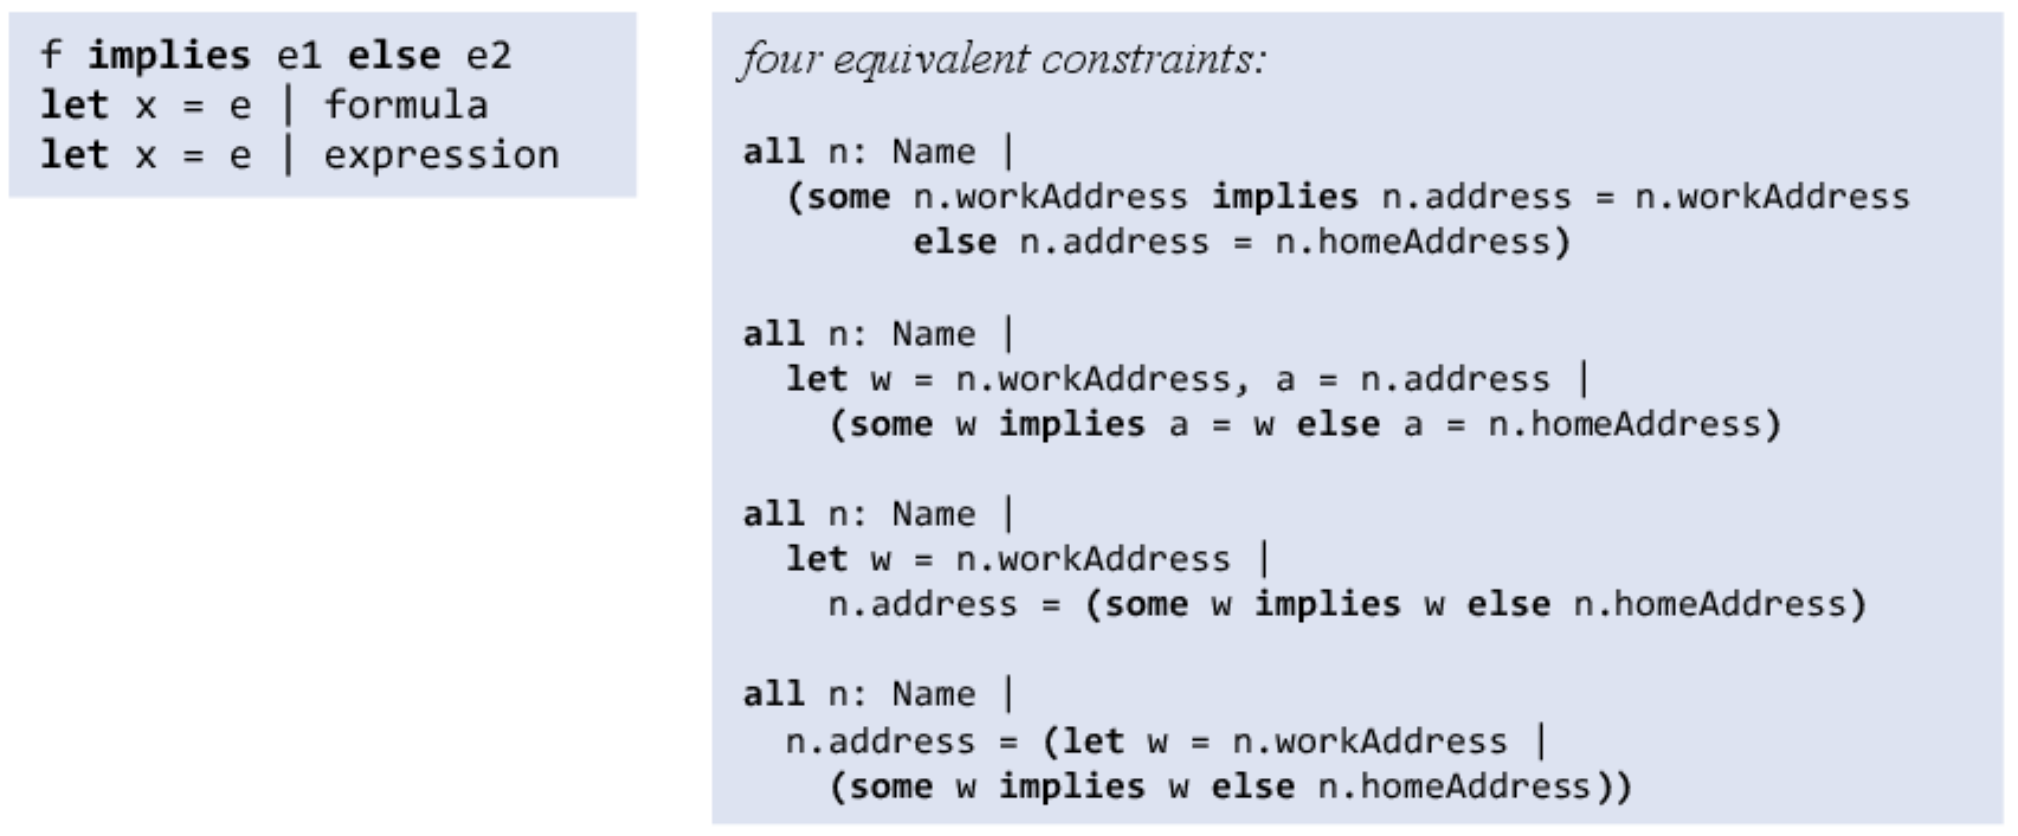
\includegraphics[width=\columnwidth]{assets/if}
\end{center}

\textbf{Cardinalities}
\begin{center}
	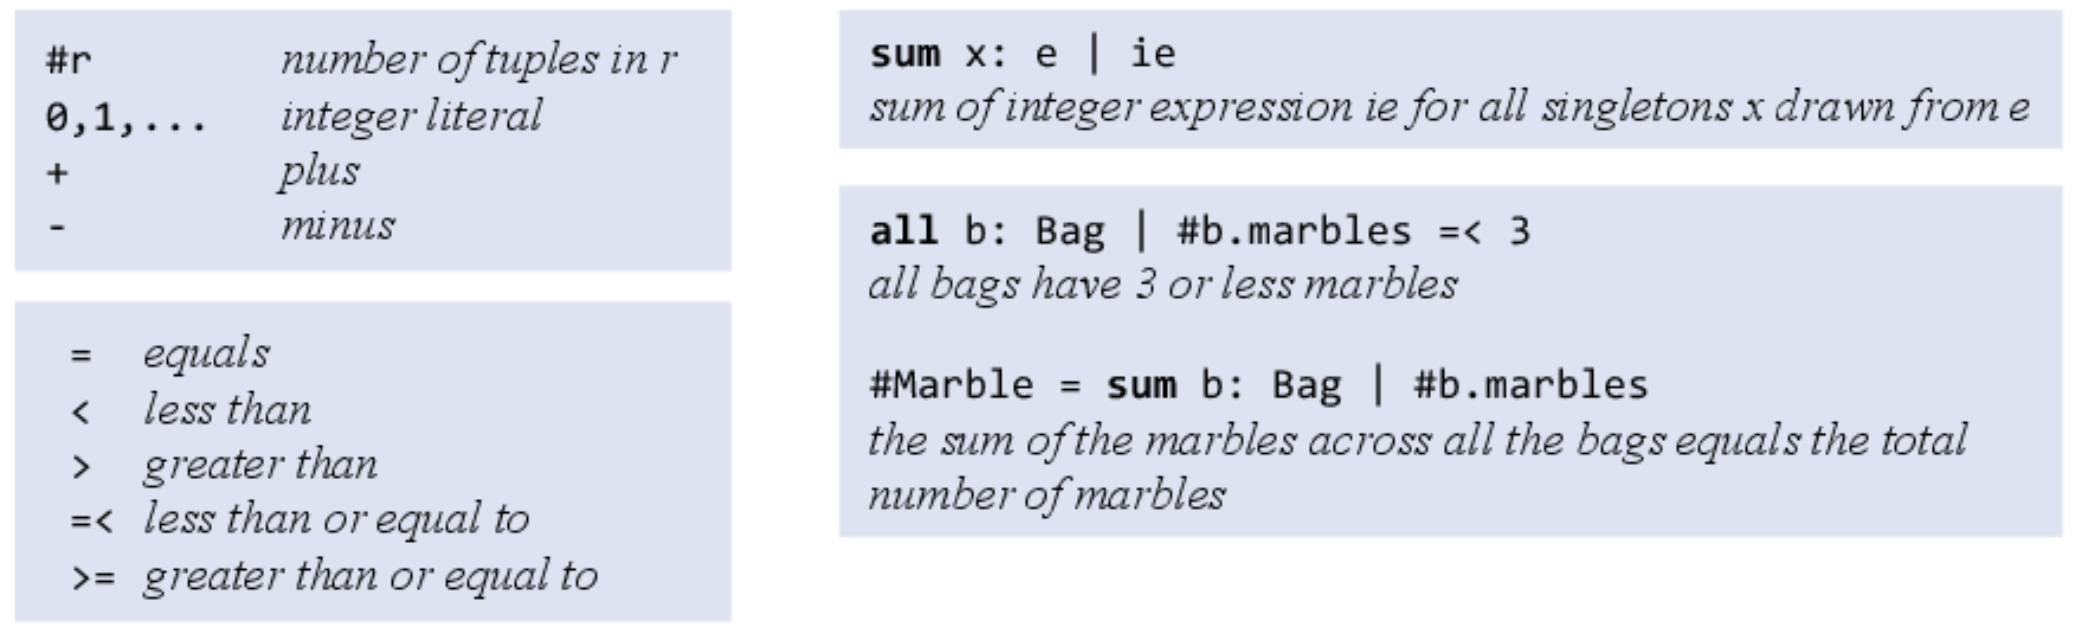
\includegraphics[width=\columnwidth]{assets/cardinalities}
\end{center}


\subsection{Static Models}

A signature declares a set of atoms (can be thought of like a class) \texttt{sig FSObject\{\}}, extends-clauses declare subset relations \texttt{sig File extends FSObject\{\}}. Like classes, signatures can be \texttt{abstract}. Further, they may constrain the cardinality of the declared set by \texttt{one, lone, some} (singleton, singleton or empty, none empty set). \\

Fields declare relations on atoms \texttt{sig A \{ f: e\}}. \texttt{f} is a binary relation on domain \texttt{A} and the range given by \texttt{e}. Range expressions may denote multiplicities \texttt{one, lone, some, set}. Fields may range over relations, with the relation declaration may including multiplicities on both sides \texttt{enrollment: Student set -> one Program}. \\

Predicates are named, parameterized formulas: \texttt{pred p[x1:e1, ..., xn:en]\{F\}}.\\

Functions are named, parameterized expressions: \texttt{fun f[x1:e1, ..., xn:en]:e \{F\}}\\

Facts add constraints that always hold, they express value and structural invariants on the model. \\

The alloy analyzer can search for structures that satisfy a constraint \texttt{C} in a model using \texttt{run C}. The existence of structures that satisfy constraints in a model is generally undecidable. The alloy analyzer searches exhaustively for structures up to a given size, therefore the problem becomes finite and decidable (e.g. \texttt{run show for 5}).\\

Exploring by manual inspection can be cumbersome. Alloy supports searching for structures that violate a given property by using \texttt{assert a \{F\}} and \texttt{check a scope}. Under-constraint models permit undesirable structures, while over-constraint models exclude desired ones.


\subsection{Dynamic Models}

Alloy 6 has a built-in notion of time based on Linear Temporal Logic (LTL). This allows us to model things like a game of ping pong. \\

LTL is boolean logic augmented with two temporal operators \texttt{next} ($X$ or $\circ$) and \texttt{until} ($U$ or $\cup$).
\begin{center}
	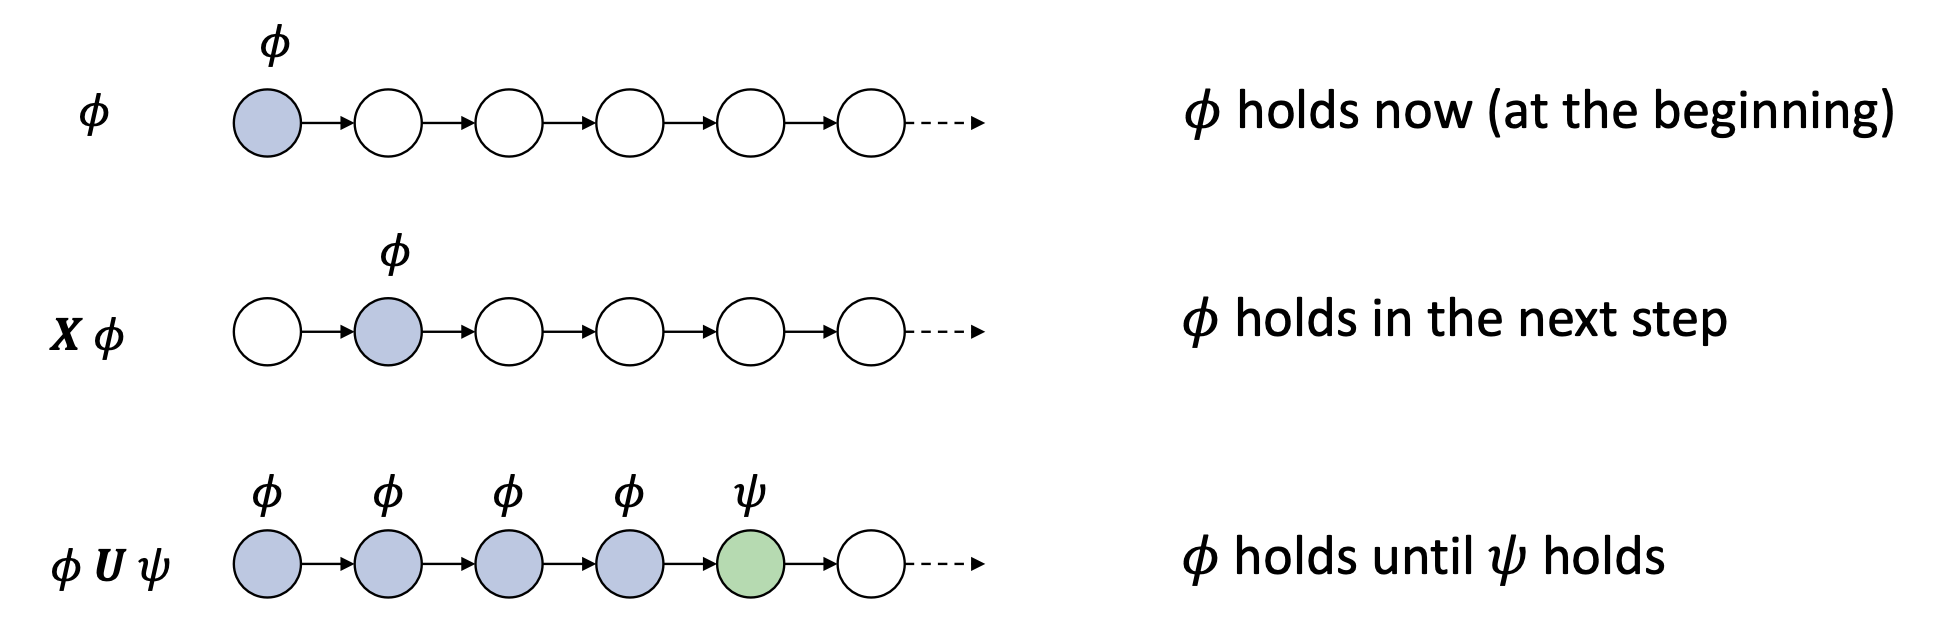
\includegraphics[width=\columnwidth]{assets/ltl}
\end{center}

From this we can derive two more operators \texttt{eventually} ($F$ or $\lozenge$) and \texttt{always} ($G$ or $\Box$). \\

Combined with mutable fields, dynamic behavior in Alloy can be summarized like this:
\begin{center}
	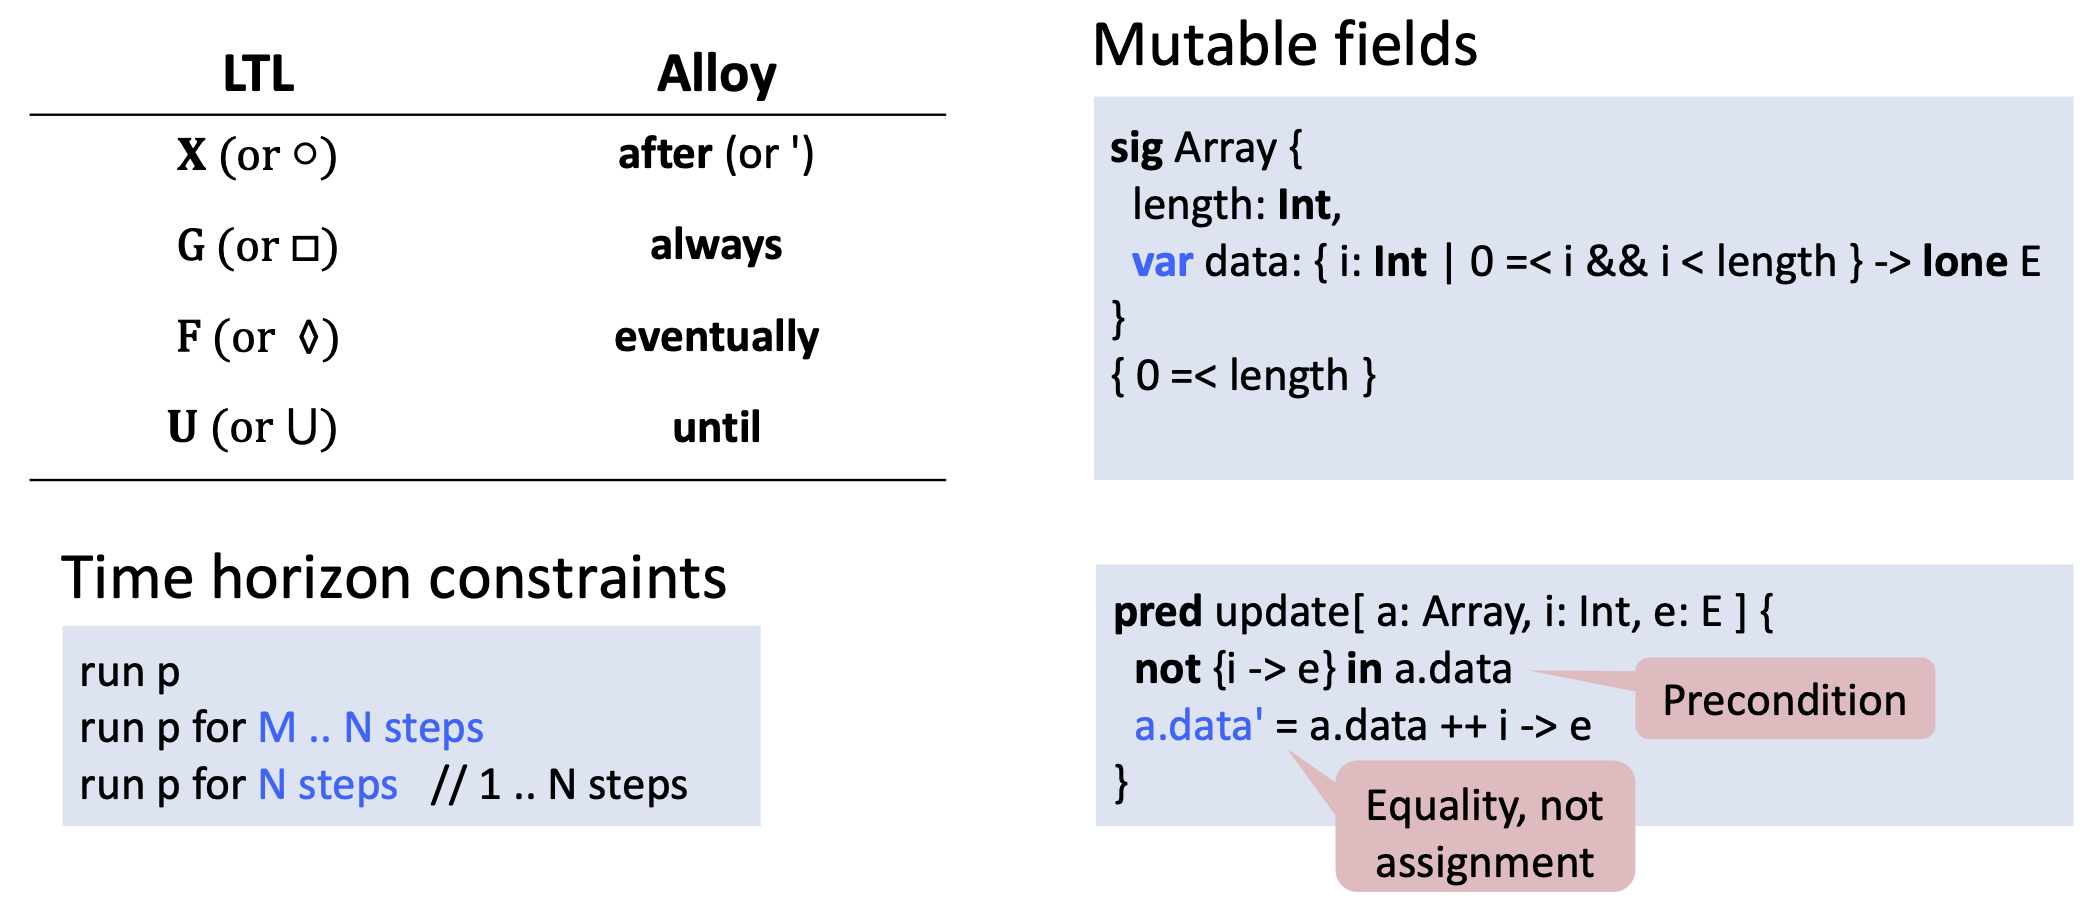
\includegraphics[width=\columnwidth]{assets/dynamic_alloy}
\end{center}

Alloy specifications are purely declarative, they describe what is done, not how it is done. Traces define the temporal behavior of the model. A first state is initialized and subsequent states are constraint using LTL operators.


\subsection{Analyzing Models}

An Alloy model specifies a collection of constraints $C$ that describe a set of structures.\\

A formula $F$ is \textbf{consistent} (satisfiable) if it evaluates to true in at leas one of these structures:
$$\exists s : C(s) \wedge F(s)$$

A formula $F$ is \textbf{valid} is it evaluates to true in all of these structures:
$$\forall s : C(s) \Rightarrow F(s)$$

Validity and consistency checking for Alloy is undecidable. The Alloy analyzer sidesteps this problem by only checking within a given scope, defining a finite bound on the size of the sets in the model. \\

In practice, SAT solvers are extremely efficient at checking consistency (performed using the \texttt{run} command). A satisfying assignment can be translated back to relations and then visualized. However, if the SAT solver returns unsatisfiable, there may exist larger structures that satisfy the conditions. \\

For validity instead of checking directly, the Alloy analyzer checks for invalidity, that is, it looks for counterexamples (performed using the \texttt{check} command).